\begin{figure}[t]
\centering
    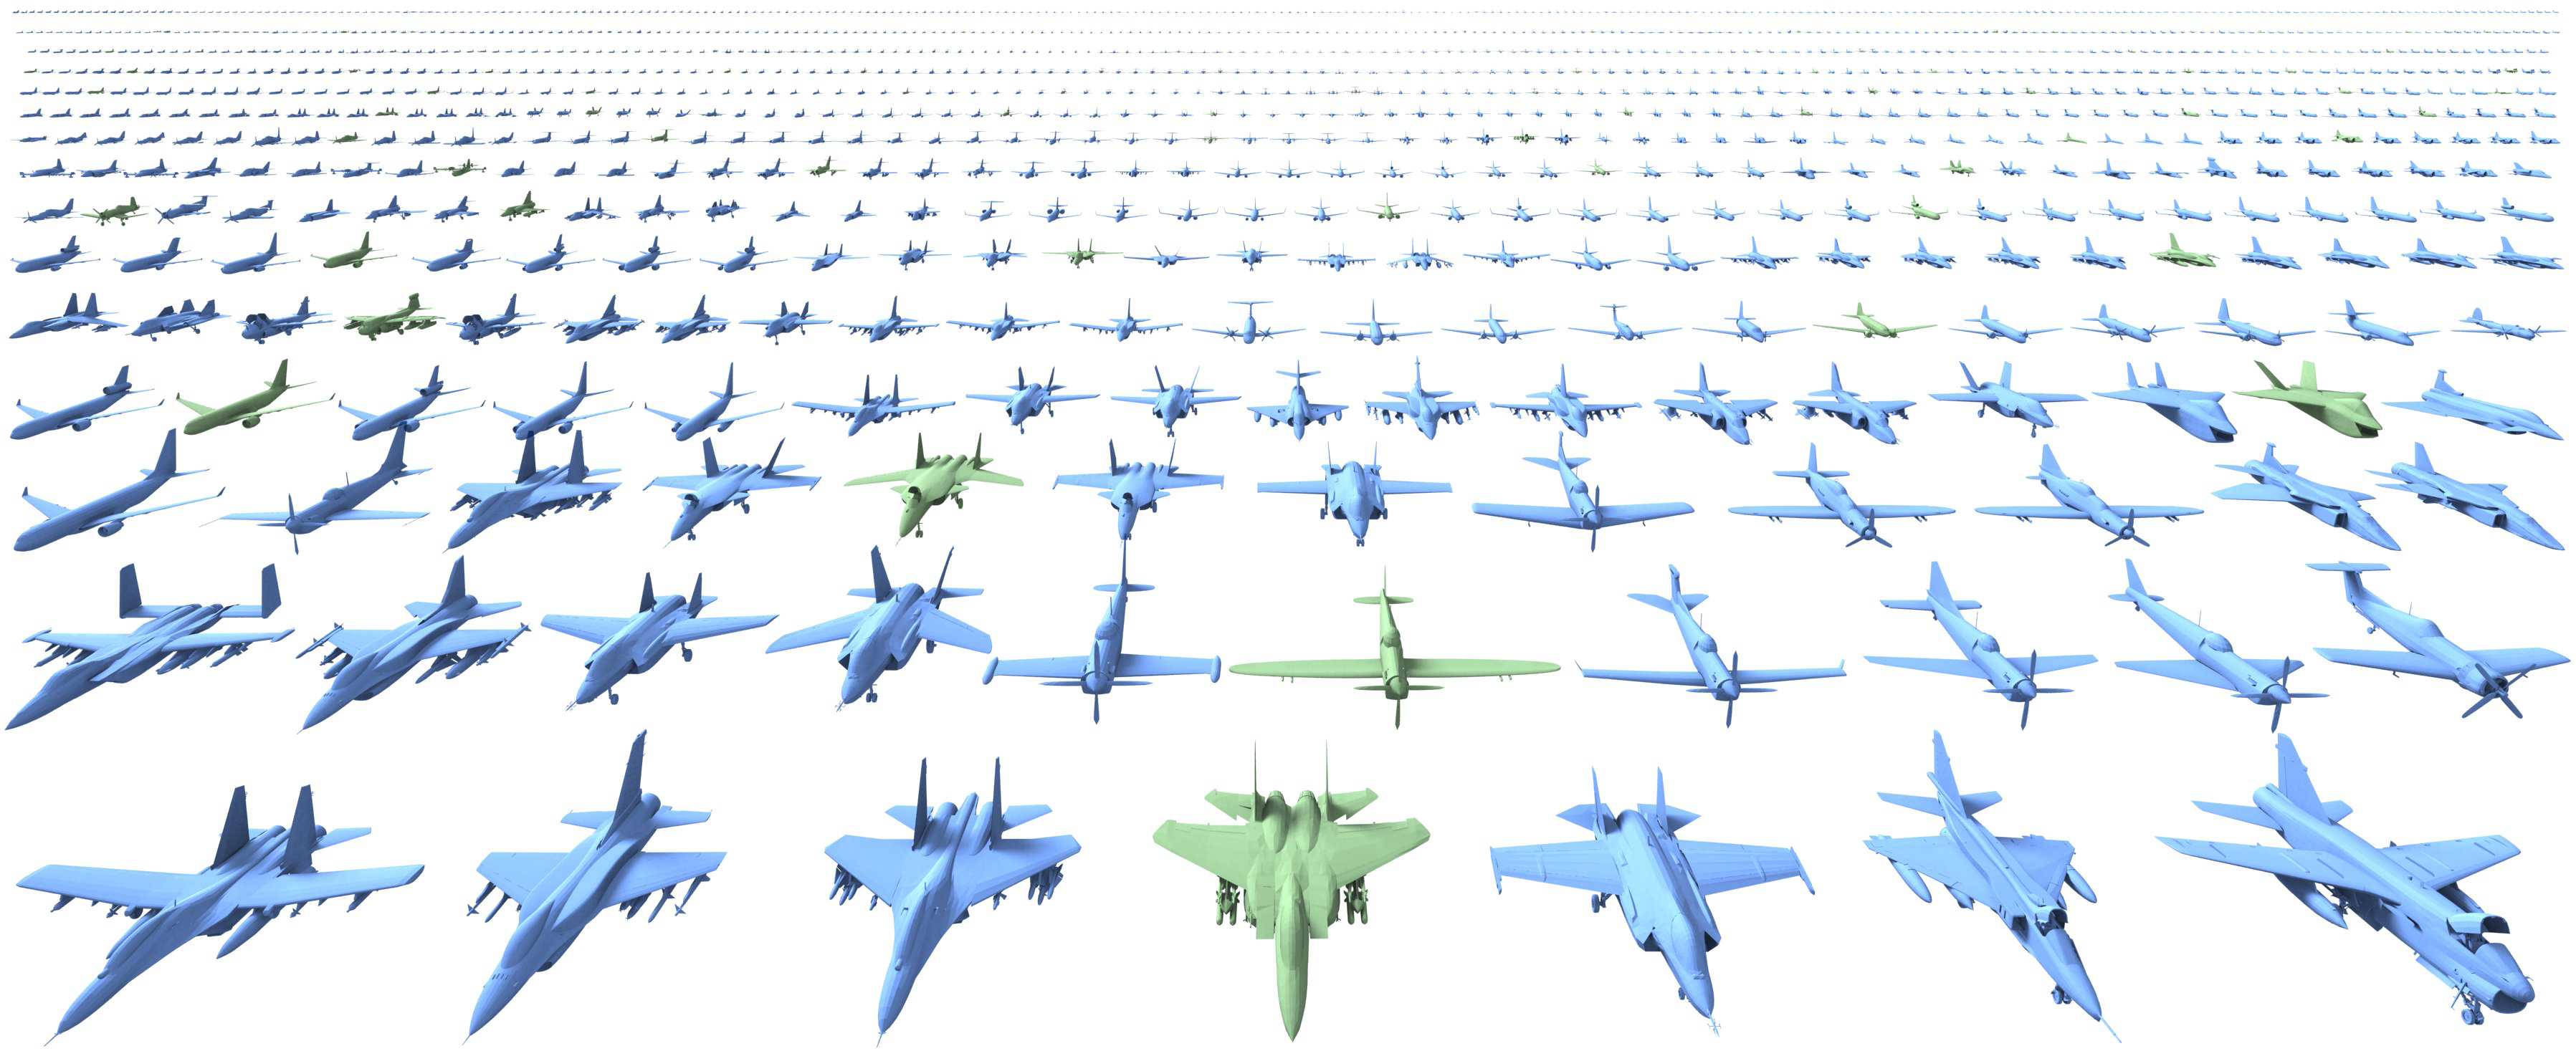
\includegraphics[width=.95\columnwidth]{fig/img/kalogerakis_sig12_synthesis}
    %\vspace{-0.3cm}
    \caption{
Given a hundred training airplanes (in green), the probabilistic model from \cite{Kalogerakis:2012:PMC} synthesizes several hundreds of new airplanes (in blue).}
    \label{fig:kalogerakis_sig12_synthesis}
\end{figure}



\rev{Many applications such as 3D games and films require large collections of 3D shapes for populating their environments. Modeling each shape individually can be tedious even with the best interactive tools. The goal of data-driven shape synthesis algorithms is to generate several shapes automatically with no or very little user supervision: users may only provide some preferences or high-level specifications to control the shape synthesis process. Existing methods achieve this task by using probabilistic generative models of shapes, evolutionary methods, or learned probabilistic grammars.}

\paragraph*{Statistical models of shapes.} The basic idea of these methods is to define a parametric shape space and then fit a probability distribution to the data points that represent the input exemplar shapes. Since the input shapes are assumed to be plausible and desired representatives of the shape space, high-probability areas of the shape space which tend to become associated with new, plausible shape variants. \rev{ This idea was first explored in the context of parametric models \cite{Blanz:1999:MMS,Allen:2003:SHB}, discussed in Section \ref{sec:recon}. By associating each principal component of the shape space defined by these methods with a Gaussian distribution, this distribution can be sampled to generate new human faces or bodies (Figure \ref{fig:allen_sig03_human}). Since the probability distribution of plausible shapes tends to be highly non-uniform in several shape classes, Talton et al. \cite{Talton:2009:EMC} use kernel density estimation with Gaussian kernels to represent plausible shape variability. The method is able to generate new shapes for tree and human body parametric spaces. }

Shapes have structure i.e., shapes vary in terms of their type and style, different shape styles have different number and type of parts, parts have various sub-parts that can be made of patches, and so on. Thus, to generate shapes in complex domains, it is important to define shape spaces over structural and geometric parameters, and capture hierarchical relationships between these parameters at different levels. Kalogerakis et al. \cite{Kalogerakis:2012:PMC} (Figure \ref{fig:kalogerakis_sig12_synthesis}) proposed a probabilistic model that represents variation and relationships of geometric descriptors and adjacency features for different part styles, as well as variation and relationships of part styles and repetitions for different shape styles. The method learns the model from a set of consistently segmented shapes. Part and shape styles are discovered based on latent variables that capture the underlying modes of shape variability. The method uses a search procedure to assemble new shapes from parts of the input shapes according to the learned probability distribution. Users can also set preferences for generating shapes from a particular shape style, with given part styles or specific parts. \fix{Instead of relying on pre-segmented shapes and high-level part descriptors to encode shape variability, Huang et al. \cite{Huang:2015:AS3} propose a probabilistic model that jointly estimates shape segmentation, surface correspondences, and surface descriptors from an input shape dataset. A deep learning procedure was used to capture hierarchical relationships of corresponding surface point positions and parts as well as their existence in the input shapes. Their probabilistic model can be sampled to directly generate point-sampled surface geometry and shape structure.}

\paragraph*{Set evolution.} \rev{Xu et al. \cite{Xu:FDS:2012} developed a method for generating shapes inspired by the theory of evolution in biology.} The basic idea of set evolution is to define cross-over and mutation operators on shapes to perform part warping and part replacement. Starting from an initial generation of shapes with part correspondences and built-in structural information such as inter-part symmetries, these operators are applied to create a new generation of shapes. A selected subset from the generation is presented via a gallery to the user who provides feedback to the system by rating them. The ratings are used to define the fitness function for the evolution. Through the evolution, the set is personalized and populated with shapes that better fit to the user. At the same time, the system explicitly maintains the diversity of the population so as to prevent it from converging into an ``elite'' set.

\paragraph*{Learned shape grammars.} Talton et al. \cite{Talton:2012:LDP} leverage techniques
from natural language processing to learn probabilistic generative grammars of shapes. The method takes as input a set of exemplar shapes represented with a scene graph specifying parent/child relationships and
relative transformations between labeled shape components. They use Bayesian inference to learn a probabilistic formal grammar that can be used to synthesize novel shapes. 